\chapter{Suggested solution}
\label{chp:suggested-solution}

In this chapter we'll walk through how the problem can be modelled and solved using linear programming.


\section{Modelling}

With some prior knowledge of graph algorithms, the first stab at solving the problem might be to look at our sample topologies and see a certain similarity to a max-flow problem -- edges have capacities, there's a set of sources, a set of sinks, and we want to maximize \emph{something}. However, there's a couple of things that make it hard to solve directly as a traditional flow problem, particularly that we don't have a single source and a single sink, but lots of them. Trying to model it as a single-source, single-sink problem quickly leads you to discover the limitations of that model, where you realize that if you actually solved, how would you be able to tell which node is generating flow on a given edge? Clearly, we need a way to distinguish node A's video from node B's video. And we need to make sure that all nodes receive video from every other node, not just maximum bitrate of \emph{any} video.

If we change perspective slightly, we see that this is not a single flow problem, but a \emph{series} of flow problems, sharing an underlying constrained resource. There's the problem of routing video from A to all other nodes, there's the problem of routing video from B to all other nodes, etc. In a conversation with $n$ participants, we now have $n$ separate flow problems, which all share the same resource. However, also this model is too limiting for our use case, as video is sent at a given bitrate, and this stream can neither be split at a given node without incurring a cost, nor does it make sense to add it; two 2Mbit videos cannot be joined to form a 4Mbit video. If you put enough restrictions on your nodes and edges it's probable that you might be able to able to prevent this from happening, but there's another way.\todo{Insert graph showing how this fails. Does it fail it any obvious way? With flow conservation on the nodes it doesn't seem like it, actually. But it might be harder to add restrictions on re-encoding later. Or it's a completely valid option, open for further investigation.}

This time around, imagine that we have a separate flow problem for each \emph{pair} of nodes; we have one problem routing node A's video to node B, we have one problem routing node A's video to node C, etc. This yields a total of $n(n-1)$ problems, which is $O(n^2)$. Modelling the problem this way means we don't have to add any supernodes to connect the targets, each node can act as sink for its own video stream, hereafter known as the \emph{commodity}, destined for itself.

One other thing we notice from our initial graph compared to traditional flow problems is that we notice that we have \emph{node constraints} in the initial graph, while flow problems only work on \emph{edge constraints}. To accommodate this, we split each node into two parts, hereafter called the external and internal part, as illustrated in \autoref{fig:node-splitting}.

\begin{figure}
    \centering
    \begin{subfigure}[t]{.48\textwidth}
        \centering
        \includegraphics[width=\textwidth]{nodesplitting-pre}
        \subcaption{Original problem}
    \end{subfigure}
    \hfill
    \begin{subfigure}[t]{.48\textwidth}
        \centering
        \includegraphics[width=\textwidth]{nodesplitting-post}
        \subcaption{Problem after node splitting}
    \end{subfigure}
    \caption{How node splitting works}
    \label{fig:node-splitting}
\end{figure}

As we now have a well-specified way to go from a given conversation to a graph that can be solved by max-flow algorithms, the entire problem can be solved by joining all the different subproblems under the same resource constraints, and solve as a multi-commodity max-flow problem. This class of problems can be solved with \gls{lp}, which can be summarized in canonical form as in \autoref{eq:lp}

\begin{align}\label{eq:lp}
    \text{maximize}\qquad &\mathbf{c^Tx} \\
    \text{subject to}\qquad &A\mathbf{x} \leq \mathbf{b} \nonumber \\
    \text{and}\qquad &\mathbf{x} \geq \mathbf{0} \nonumber
\end{align}

The vector $\mathbf{x}$ is the variables we're trying to find a solution for, each entry in the vector defines a flow on a given edge in the graph. The vector $\mathbf{c}$ scores each flow to determine the total gain, while the matrix $A$ is the set of constraints put on the system, like staying below bandwidth, flow conversation among non-source and non-sink nodes, and so on.

As \gls{lp} is a well-known and very general technique that's effective to a vast collection of problems, there are lots of LP-solvers freely available\footnote{\url{https://en.wikipedia.org/wiki/Linear_programming\#Solvers_and_scripting_.28programming.29_languages}}. This simplifies building a solution on top of \gls{lp}; if you can model your problem as a linear program, it can be efficiently solved by existing, well-tested code. For our experimental solution we chose a solver somewhat arbitrarily among those which had Python bindings, and picked \gls{glpk}.


\section{Maximization}

Then there's the issue of the \emph{something} we wanted to maximize in the problem. If you want to consider the full picture with users influenced by mood, context and lots of other human factors that come into play, this is a complex topic that could warrant several papers on its own. In this thesis we'll simplify the problem to only consider two factors that influence our decision: bandwidth and latency. Thus, our reformulated problem is to \emph{maximize} bandwidth of each commodity at a \emph{minimal} latency. Formulated for each node in a conversation, this becomes our \emph{objective function}. The weighting between the two can be parametrized and left for implementations to decide.

Given those factors, our problem is solved by finding a solution to the problem in \autoref{eq:objective}, where $x^k$ is a matrix with the amount of commodity $k$ transmitted on each edge, $c(i, j)$ is a cost function for the edge between $i$ and $j$, and $g_i$ is a vector of how much each device has to gain from receiving something. The gain is reflected in the device types, a phone will require less bandwidth to satisfy the user than a desktop computer with a large display will, thus introducing the gain makes sure the system will allocate bandwidth to each device's potential and capability. $s_k$ and $t_k$ is the source and sink for commodity $k$, $d_k$ is the gain. $u_{i, j}$ is the capacity of the link between $i$ and $j$.

\begin{gather}\label{eq:objective}
    max \sum_{k \in K} (d_{t_k} \sum_{w \in V} log(x_{w, t_k}^k) - \sum_e 1 + 1/(u_e - x_e^k))\\
    \text{subject to} \nonumber \\
    \sum_{k \in K} \sum_{(i, j) \in E} x_{i, j}^k = 0, \qquad{} i, j \neq s_k, t_k \\ \label{eq:bwlim}
    \sum_i \sum_j (\sum_{k \in K}x_{i, j}^k) < u_{i, j}
\end{gather}


In plain English: For each commodity, maximize the gain of sending that commodity to it's receiver, minus the link cost sending said commodity induces, while all nodes conserve bandwidth except the source and sink for a commodity (\autoref{eq:bqlim}) and no link exceeds its capacity. The observant reader will note that we require each sink to receive each commodity, instead of having each source send each commodity. We'll come back to this decision in \autoref{sec:repeaters}

In any case, this raises some other issues that has to be handled. The objective function has to be linear to be solved as a linear program, but several of our parameters are non-linear. Perceived gain from increasing bandwidth is non-linear, the cost of link utilization is non-linear, and perceived gain from reducing latency is probably non-linear. However, all of these can be approximated arbitrarily close by a piecewise linear function, as illustrated in \todo{Insert example of piecewise linear functions}. This too can be parametrized, as either the number of pieces to divide into or as the maximum deviation from the true allowed.

These different cases will be discussed in the following paragraphs, before we arrive at our final objective function.


\section{Perceived Gain From Bandwidth}

Increasing the bitrate of video is subject to diminishing returns, increasing the bitrate from 1Mbps to 2Mpbs yields a bigger return for the user than going from 4Mbps to 5Mbps. x264, the H.264 encoder powering applications like VLC\footnote{\url{http://www.videolan.org/developers/x264.html}}, HandBrake\footnote{\url{https://handbrake.fr/}} and ffmpeg\footnote{\url{https://trac.ffmpeg.org/wiki/Encode/H.264}}, uses an exponential scale for the relationship between bitrate and perceived quality\footnote{\url{https://trac.ffmpeg.org/wiki/Encode/H.264\#crf}}, as illustrated in \autoref{fig:bitrate-quality}.\todo{make pretty}

\begin{figure}
    \centering

    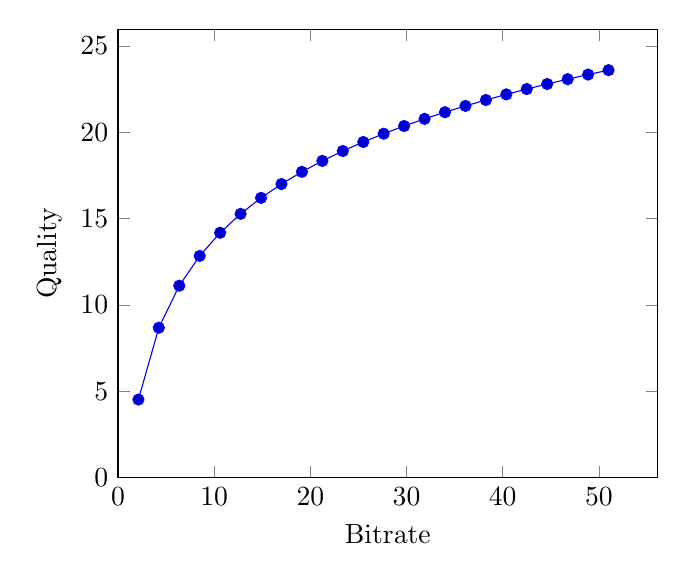
\begin{tikzpicture}
        \begin{axis}[
            xlabel={Bitrate},
            ylabel={Quality},
            xmin=0,
            ymin=0,
            inner axis line style={=>}
        ]

        \addplot+[domain=0:51]{6*ln(x)};
        \end{axis}
    \end{tikzpicture}

    \caption{The relationship between bitrate and quality in the x264 project}
    \label{fig:bitrate-quality}
\end{figure}

With a linear gain from increased bandwidth, bumping traffic from a given node from 4Mbps to 5Mbps would yield the same return as bumping another node from 1Mbps to 2Mbps, and thus the algorithm would be unlikely to find a fair allocation of bandwidth. Encoding diminishing returns into the objective function ensures that everyone will be allocated a fair share, and still allows nodes with excess bandwidth to grow further than more constrained nodes.

\todo{Figure out how to actually get this into the objective}


\section{Link Utilization}

The cost of utilizing a given network link is a function of the link's utilization, which is given by the queuing delay formula, $1/(1 - \mu/\lambda)$. As can be seen in \autoref{fig:utility-latency}, this function is not linear, and can thus not be used directly in our objective function. Nonetheless, we can achieve the same goal -- punishing over-utilization of individual links -- by approximating the function with a piecewise linear function. Conceptually, we can imagine that instead of a single link going into a node, there's a \emph{set} of links to each node, with exponentially increasing costs. Thus a 8Mbps link might be divided into four links of 2Mbps, with exponentially increasing costs.

Assuming that the weighting between the segments follows the queuing delay formula given above, the ratio between the extra punishment for using the last 10\% of a link and the gain from increasing bandwidth by those extra 10\% can be tuned by implementations. This ratio would basically be a measure of how heavily to hit the network to gain maximum quality. To avoid excessive packet loss, link utilization should probably not exceed 90\%, which can also be achieved by under-reporting the actual bandwidth to the algorithm. What the effects of that would be, compared to increasing the ratio towards more heavily punishing excessive link utilization, is unknown and requires more study to say anything conclusive about.

\todo{Insert partitioning-algo here}

Based on this formula, we can formulate the cost multiplier of a link as $1 + k/(\mu - \lambda)$, where $k$ is a customizable parameter for how heavily link saturation should be punished. In our experiments, $k=10$ seems appropriate. This cost function can be seen in \autoref{fig:utility-latency}. We then partition this function into a small set of piecewise linear intervals, which we can model as parallel edges between two nodes, with different capacities and costs. Keeping this set small limits the number of variables in the resulting matrix, and thus keeps processing times reasonably low.

\begin{figure}
    \centering
    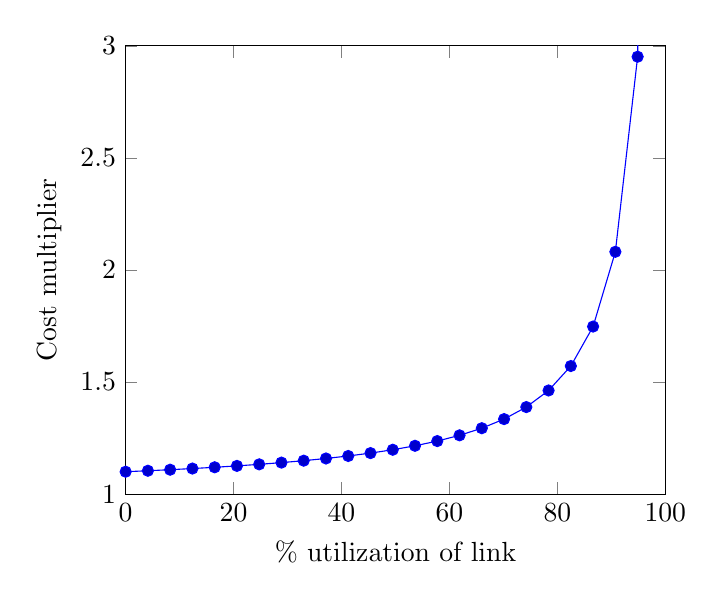
\begin{tikzpicture}
        \begin{axis}[
            xlabel={\% utilization of link},
            ylabel={Cost multiplier},
            xmin=0,
            ymin=1,
            ymax=3,
            xmax=100]

        \addplot+[domain=0:99]{1 + 10/(100 - x)};
        \label{fig:utility-latency}
        \end{axis}
    \end{tikzpicture}
    \caption{How packet delay grows as a function of link utilization for network links. Packet delay for us is equivalent to cost, which thus has to be approximated in an implementation.}
    \label{fig:utility-latency}
\end{figure}


\begin{center}
    \label{tab:utilization-to-cost}
    \begin{tabular}{| l | l |}
    \hline
    \textbf{Link utilization} & \textbf{Cost multiplier} \\ \hline
    0--50\% & 1.2 \\ \hline
    51--75\% & 1.40 \\ \hline
    76--80\% & 1.50 \\ \hline
    81--90\% & 2.00 \\ \hline
    \end{tabular}
\end{center}

Using this partitioning as a guide, we can map any number of slots on a physical link into a set of edges $E$ in our graph where $|E| <= 4$.




\subsection{Alternative model}

One alternative way to model the problem, is to skip the node splitting step of the previous model, and instead connect nodes directly, but stay below bandwidth by adding constraints for the total sum going out from each node. Which model to choose is -- as in every engineering matter -- a question of priorities. The first model is a bit harder to comprehend initially, but results in fewer total edges than the latter model does when $n>3$, as can be seen in \autoref{fig:model-scaling}. Edge counts do not matter that much when $n$ is low as finding a solution will occur in trivial time anyway, but the difference might be substantial when n is larger. \todo{If performance ends up being an issue for larger graphs, add a note here about more research being needed into optimizing performance, as alternative models might be an avenue to explore for achieving that.}

\begin{figure}
\centering
    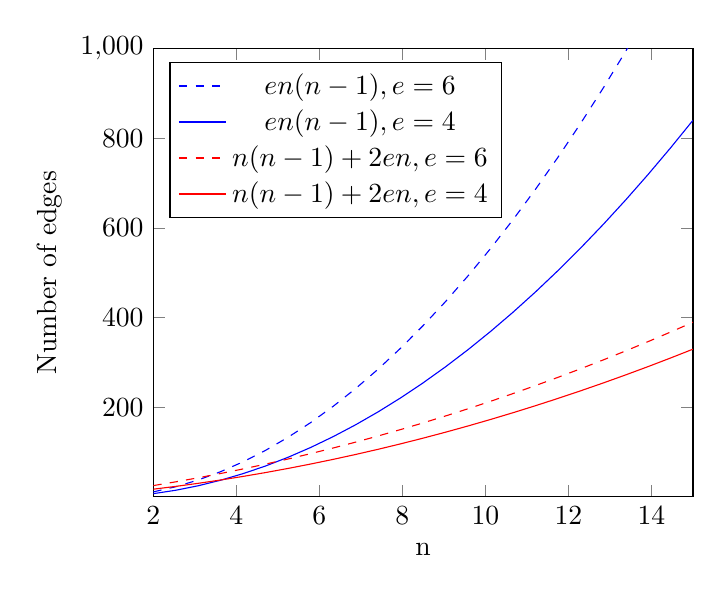
\begin{tikzpicture}
        \begin{axis}[
            xlabel={n},
            ylabel={Number of edges},
            xlabel near ticks,
            ylabel near ticks,
            legend pos=north west,
            xmin=2,
            ymin=1,
            ymax=1000,
            xmax=15]

        \addplot+[dashed, domain=2:15, mark=none, color=blue]{6*x*(x-1)};
        \addlegendentry{$en(n-1), e=6$}

        \addplot+[domain=2:15, mark=none, color=blue]{4*x*(x-1)};
        \addlegendentry{$en(n-1), e=4$}

        \addplot+[dashed, domain=2:15, mark=none, color=red]{x*(x-1) + 2*x*6};
        \addlegendentry{$n(n-1) + 2en, e=6$ }

        \addplot+[domain=2:15, mark=none, color=red]{x*(x-1) + 2*x*4};
        \addlegendentry{$n(n-1) + 2en, e=4$ }
        \label{fig:utility-latency}
        \end{axis}
    \end{tikzpicture}
    \caption{How the number of edges in the graph scales for different modeling techniques.}
    \label{fig:model-scaling}
\end{figure}


\section{Repeaters}\label{sec:repeaters}

This is all well and good, but solving our problem as we've posed it so far will only yield us something very close to what browsers figure out by trial and failure today. However, where today's solutions are topology-bound, we can go beyond those limitations, and use our established technique on slightly modified flow networks.

One thing we note with pure peer-to-peer topologies, is that required bandwidth in and out grows linearly with $n$, which quickly saturates constrained nodes. Going pure peer-to-peer is most often optimal in terms of latency, but if the necessary bandwidth is not available, we want to have the option to fall back to relaying some -- but not necessarily all -- nodes some unconstrained repeater. This repeater could be provided by the service provider in a datacenter somewhere, or could be one of the other nodes in the conversation with excess bandwidth available\footnote{These are the nodes Skype referred to as "supernodes"}. We have assumed that repeaters are provided in datacenters for now, but the constraints can easily be adapted to accomodate nodes as repeaters in a conversation.

Formulating the constraints get a bit weird for repeaters, as they \emph{do not} conserve either bandwidth or commodities. We say that repeaters can \emph{mangle} commodities, which means it can receive the commodity $k$ sent from node A to node B, and can send it as commodity $k$ to B, but it can also send it as commodity $m$ to node C, assuming $m$ is the commodity sent by node A to node C. This is less awkward if the alternative model suggested in \section{sec:alternative-model} is implemented, but there was only time to implement one model for this thesis, so that is left as excercise for the reader.

There is some constraints on repeaters though, namely that the incoming amount of one commodity has to be equal to the outgoing amount of all other commodities from the same source. Practically speaking, repeaters can not change the bitrate of incoming video, either up or down. That way, a repeater is a pure IO-bound device, which does not require much else than a fast Internet connection to be operated.

Note that since commodities are routed independently in our flow network, it's possible for a node to use a repeater only for outgoing traffic, but still receive incoming traffic directly from its peers. This will probably often be the case, as many consumer connections are still highly asymmetric in inbound/outbound capacity.

Repeaters are also practical since they're not required to know the contents of the packages it forwards, and thus anyone with spare bandwidth can provide a repeater for anyone to use, without compromising the confidentiality of those conversations.

Deployment wise, repeaters are very similar to \gls{turn}-servers, which are used for \gls{nat}-traversal by relaying all video through a central server. A repeater could probably re-use much of the \gls{turn}-protocol, the only practical difference being that a repeater is one-to-many, while TURN is one-to-one.


\section{Transcoders}

Another unit that can be added to the flow network is a transcoder, which is like a repeater in that it has practically unconstrained bandwidth in and out, but also has the capability to transcode incoming video. If node A only has 2Mbps upload capacity, and node B is a desktop with 10Mbps downlink, and node C is a phone with only 1 Mbps downlink, A can send its full 2Mbps video stream to a transcoder, which can then forward the full 2Mbps stream to node B, but transcode the stream down to a leaner 1Mbps stream for node C. That way A is able to fully utilize its upload capacity, while the receivers get a stream best utilizing their downlink capacity.

Transcoders are more costly to run than transcoders, due to much heavier compute operations required to transcode video in realtime. They will typically be nodes with specialized hardware for video encoding, such as Intel processors with Quick Sync\footnote{Intel's hardware-accelerated H.264 encoder, first introduced in the Sandy Brigde family of CPUs}, GPUs, or other hardware built for real-time streaming.

Constraint-wise, a transcoder performs the same commodity mangling as repeaters, but can output commodities of arbitrary bitrates less than or equal to the source commodity.

However, in contrast to repeaters, transcoders have to access the contents of the calls to be able to transcode the signal. This will be the case until a homomorphic cryptosystem is available for video transcoding, which might be in a couple of years or it might be never. Here's crossing some fingers.


\section{The Algorithm}

Given the model, how do you efficiently find the "best" topology?


\section{Implementation}\label{sec:implementation}

\todo{Write about how the implementation was done}


\section{Tuning}

How can the algorithm be tuned, and how was the parameters chosen?
